\documentclass[12pt,a4paper]{report}
\usepackage{graphicx}
\usepackage{amsmath}
\usepackage{fancyhdr}
\usepackage{cite}
\usepackage{framed}
\usepackage{a4wide}
\usepackage{float}
\usepackage{epsfig}
\usepackage{longtable}
\usepackage{enumerate}
\usepackage{afterpage}
\usepackage{multirow}
\usepackage{ragged2e}
\usepackage{gensymb}
\usepackage{amsfonts} 
\usepackage[left=3.5cm,top=1.5cm,right=3cm,bottom=4cm]{geometry}
\usepackage{setspace}           
\usepackage{float}
\usepackage{txfonts}
\usepackage{lipsum}
\newcommand{\Usefont}[1]{\fontfamily{#1}\selectfont}
\usepackage{lscape} % for landscape tables
\renewcommand{\baselinestretch}{1.7} 
\usepackage{blindtext}
\usepackage{xpatch}
\usepackage{url}
\usepackage{leqno}
\usepackage{subcaption}
\linespread{1.5}
\usepackage[intoc, english]{nomencl}
\hyphenpenalty=5000
\tolerance=1000
\usepackage[nottoc]{tocbibind}
\bibliographystyle{IEEEtran}
\renewcommand{\bibname}{References}
%*******************************************************************
%                        Header and Footer   
% This is not required in Technical reports submitted to CET ECE department.
% Please leave it commented                       
%*******************************************************************
%\pagestyle{fancy}
%\fancyhead{}
%\header and footer section
%\renewcommand\headrulewidth{0.1pt}
%\fancyhead[L]{\footnotesize \leftmark}
%\fancyhead[R]{\footnotesize \thepage}
%\renewcommand\headrulewidth{0pt}
%\fancyfoot[R]{\small Government Engineering College Trivandrum}
%\renewcommand\footrulewidth{0.1pt}
%\fancyfoot[C]{2020 - 2021}
%\fancyfoot[L]{\small Title of the Seminar/Project}
%*******************************************************************
%*********************Figures*****************************
% Save all figures in the folder figures and include them in your 
% report using the command \includegraphics{figure-name}

\graphicspath{{figures/}}

% figure files can be in jpeg,jpg, png or pdf formats
%*******************************************************************
\begin{document}
	
%****The entries in this section are to be filled in by the student with appropriate values *************

% These values are used thoroughout the report 
% please fill in the appropriate values
\gdef \title{Constructing an Associative Memory System Using Spiking Neural Network} % Seminar title
\gdef \author{SANKAR VINAYAK E P}	 %student name
\gdef \dept{Computer Science and Engineering} %Department
\gdef \degree{Bachelor of Technology} %degree
\gdef \branch{Computer Science and Engineering} %branch
\gdef \college{Government Engineering College}
\gdef \collegeplace{Sreekrishnapuram}
\gdef \rollno{PKD19CS046} %KTU Reg No
\gdef \deptabbr{Dept.of CSE} %Dept name abbreviation

\gdef \guide{Liji L Dominic} %Seminar guide
\gdef \guidedes{Assistant Professor}%Seminar guide designation

\gdef \semcordinatorA{Dr. Swaraj K P}% Seminar coordinator 1 
\gdef \semcordinatorAdes{Associate Professor}% Seminar coordinator 1 designation

\gdef \semcordinatorB{Prof. Seminar coordinator 2} % Seminar coordinator 2 
\gdef \semcordinatorBdes{Associate Professor}% Seminar coordinator 2 designation

\gdef \hod{Dr. Sabitha S} %Head of Department
\gdef \hoddes{Professor and Head} %HOD designation

\gdef \acadyear{2022 - 23} % Academic year
\gdef \month{DECEMBER 2022} %Month of Report submission
\gdef \date{15-12-2022} %Date of signing the declaration

%*******************************************************************
% The font pages. The source tex files are there in the folder
%==================================coverpage.tex================================


\newenvironment{coverpage}
\thispagestyle{empty}
\begin{titlepage}
	\begin{center}
		\vspace*{5pt}
		{\Usefont{phv} \Large \bf \title \par}
		\vspace*{20pt}
		\large { 
			A Seminar Report \par
			submitted by\\
		{\bf\author}\\
		{\bf\rollno}\\
			to \\
			the APJ Abdul Kalam Technological University\\
			in partial fulfillment of requirements for the award of degree}\\ [.15\baselineskip] \par of \\
		\Usefont{ppl} {\bfseries  \degree}\\
		in\\
		{\Usefont{ppl} {\bfseries \branch}}\\
		
		\vspace*{30pt}
		\centering
		\begin{figure}[h!]
			\centerline{
\includegraphics[scale=0.4]{logo.png}}
		\end{figure}
		
		\vspace{\stretch{0.5}}
		\footnotesize{\bf DEPARTMENT OF COMPUTER SCIENCE AND ENGINEERING} \par
		\bf{GOVERNMENT ENGINEERING COLLEGE PALAKKAD} \par
		\bf{SREEKRISHNAPURAM 678 633} \par
		\bf{\month}
	\end{center}		
\end{titlepage}	
 %Unless essential Do not edit this tex file



%%********************Certificate*******************

% To print name of only the seminar coordinator 1 in the certificate page
%==================================certificate1.tex================================
% To print name of only the seminar coordinator 1 in the certificate page

\newenvironment{certificate1}

	\newpage
	\begin{center}	
		%\vspace{1.5cm}
		
		\textbf{DEPT. OF COMPUTER SCIENCE ENGINEERING}	
		\textbf{GOVRNMENT ENGINEERING COLLEGE}	
		\textbf{PALAKKAD}
		
		\textbf{\acadyear} 
	\end{center}
	
	
	\begin{center}
		
\includegraphics[scale=0.3]{logo}	
	\end{center}
	\begin{center}
		\textbf{CERTIFICATE}
	\end{center}
	
	This is to certify that the report entitled \textbf{\title} submitted by \textbf{\author}\hspace*{2pt}(\rollno), to the APJ Abdul Kalam Technological University in partial fulfillment of the B.Tech.\ degree in \branch \hspace*{2pt} is a bonafide record of the seminar work carried out by him under our guidance and supervision. This report in any form has not been submitted to any other University or Institute for any purpose.
	
	
	\begin{singlespace}
		\vspace*{1cm}
		\begin{table}[h!]
			\centering
			\begin{tabular}{p{7cm} p{1.5cm} p{7cm}} 
				\textbf{\guide} && \textbf{\semcordinatorA} \\
				(Seminar Guide) &&  (Seminar Coordinator)\\
				\guidedes & & \semcordinatorAdes\\ 
				Dept.of CSE && Dept.of CSE\\ 
				GOVRNMENT ENGINEERING  & &GOVRNMENT ENGINEERING \\
				COLLEGE PALAKKAD && COLLEGE PALAKKAD\\
			\end{tabular}
			
		\end{table}
		
		\vspace*{1.3cm}
		
		\begin{center}
			
			%\hline
			\textbf{\hod} \\ 
			\hoddes\\ 
			Dept.of CSE\\ 
			GOVRNMENT ENGINEERING COLLEGE\\
			PALAKKAD\\
			
		\end{center}
	\end{singlespace}
	
	\thispagestyle{empty}



 

% To print names of both the seminar coordinators in the certificate page
%%==================================certificate2.tex================================
% To print names of both the seminar coordinators in the certificate page
\newenvironment{certificate2}

\newpage
\begin{center}	
	%\vspace{1.5cm}
	
	\textbf{DEPT. OF ELECTRONICS \& COMMUNICATION ENGINEERING}	
	\textbf{COLLEGE OF ENGINEERING}	
	\textbf{TRIVANDRUM}
	
	\textbf{\acadyear} 
\end{center}

\begin{center}
	
\includegraphics[scale=0.5]{cet_logo}	
\end{center}
\begin{center}
	\textbf{CERTIFICATE}
\end{center}

This is to certify that the report entitled \textbf{\title} submitted by \textbf{\author} \hspace*{2pt}(\rollno), to the APJ Abdul Kalam Technological University in partial fulfillment of the B.Tech.\ degree in \branch \hspace*{2pt} is a bonafide record of the seminar work carried out by him under our guidance and supervision. This report in any form has not been submitted to any other University or Institute for any purpose.


\begin{singlespace}
	\vspace*{2cm}
	\begin{table}[h!]
		\centering
		\begin{tabular}{p{7cm} p{0.9cm} p{7cm}} 
			\textbf{\guide} && \textbf{\semcordinatorA} \\
			(Seminar Guide) &&  (Seminar Coordinator)\\
			\guidedes & & \semcordinatorAdes\\ 
			\deptabbr && \deptabbr\\ 
			\college & &\college\\
			\collegeplace && \collegeplace\\
		\end{tabular}
		
	\end{table}
	
	\vspace*{1.3cm}
	
	\begin{center}
		\begin{tabular}{p{7cm} p{0.9cm} p{7cm}} 
			%\hline
			\textbf{\semcordinatorB} && \textbf{\hod} \\
			\semcordinatorBdes & & \hoddes\\ 
			\deptabbr && \deptabbr\\ 
			\college & &\college\\
			\collegeplace && \collegeplace\\
		\end{tabular}
	\end{center}
\end{singlespace}

\thispagestyle{empty}



 %Please uncomment this and comment the previous line

%%***************************************************


%==================================declaration.tex================================
%
\newpage
\newenvironment{declaration}
\thispagestyle{empty}
\chapter*{DECLARATION}
% \begin{center}
%     \vspace*{30pt}
%     \textbf{DECLARATION}\\
% \end{center}
I \author \hspace*{2pt} hereby declare that the seminar report {\bf{\title}}, submitted for partial fulfillment of the requirements for the award of degree of Bachelor of Technology of the APJ Abdul Kalam Technological University, Kerala is a bonafide work done by me under supervision of \guide \hspace*{2pt} \par
This submission represents my ideas in my own words and where ideas or words of
others have been included, I have adequately and accurately cited and
referenced the original sources.\par
I also declare that I have adhered to ethics of academic honesty and integrity
and have not misrepresented or fabricated any data or idea or fact or source in
my submission. I understand that any violation of the above will be a cause for
disciplinary action by the institute and/or the University and can also evoke
penal action from the sources which have thus not been properly cited or from
whom proper permission has not been obtained. This report has not been
previously formed the basis for the award of any degree, diploma or similar
title of any other University.

\noindent \begin{minipage}{0.45\linewidth}
    \begin{flushleft}
        \vspace{4cm}

        \collegeplace \\
        \date

    \end{flushleft}
\end{minipage}
\hfill
\begin{minipage}{0.45\linewidth}
    \begin{flushright}
        \vspace{4cm}

        \author\\

    \end{flushright}
\end{minipage}
\thispagestyle{empty} %Unless essential Do not edit this tex file

\pagenumbering{roman} 
%%***************************************************
% Default Acknowledgement page
%==================================acknowledgement.tex=============================
\chapter*{\centering Acknowledgement}%
\addcontentsline{toc}{chapter}{Acknowledgement}%

%\newenvironment{acknowledgement}

I take this opportunity to express my deepest sense of gratitude and sincere
thanks to everyone who helped me to complete this work successfully. I express
my sincere thanks to \textbf{ \hod}, Head of Department, \dept,
\college\hspace*{2pt} \collegeplace \hspace*{2pt} for providing me with all the
necessary facilities and support.\par

I would like to express my sincere gratitude to \textbf{\semcordinatorA} and
\textbf{\semcordinatorB}, \hspace*{2pt} department of \hspace*{2pt} \dept,
\hspace*{2pt} \college \hspace*{2pt} \collegeplace \hspace*{2pt} for their
support and co-operation.

\noindent I would like to place on record my sincere gratitude to my seminar guide \textbf{\guide},\hspace*{2pt}\guidedes,\hspace*{2pt}\dept,\hspace*{2pt}\college \hspace*{2pt} for the guidance and mentorship throughout the course.

Finally I thank my family, and friends who contributed to the succesful
fulfilment of this seminar work.

\vspace*{30pt}
\begin{flushright}
	\textbf{\author}
\end{flushright}
\thispagestyle{plain}  %Unless essential Do not edit this tex file

%%********************************Abstract***********************
%============================= abstract.tex================================
\chapter*{\centering Abstract}%
%\addcontentsline{toc}{chapter}{\numberline{}Abstract}%
\begin{center}
    \addcontentsline{toc}{chapter}{Abstract}%
\end{center}

An associative memory system is a type of artificial neural network that can
learn and store associations between input and output patterns. Spiking neural
networks, on the other hand, are a type of neural network that models the
behaviour of neurons in the brain by using discrete time steps to simulate the
firing of individual neurons. Combining these two concepts can result in an
effective memory representation technique in which the contents can be accessed
with speed and efficiency. The report provides an overview of the principles of
associative memory and spiking neural networks, and then describe the
architecture and training procedure for the system. The results show that
spiking neural networks can be effective for implementing associative memory
systems, and have potential applications in a range of computational
neuroscience and machine learning problems.

% The aim of this seminar report is to explore the use of spiking neural networks
% for the construction of associative memory systems. An associative memory
% system is a type of artificial neural network that is able to learn and store
% associations between input and output patterns. Spiking neural networks, on the
% other hand, are a type of neural network that models the behavior of neurons in
% the brain by using discrete time steps to simulate the firing of individual
% neurons. In this report, we will discuss the principles behind both associative
% memory systems and spiking neural networks, and describe how they can be
% combined to create a powerful and efficient associative memory system. We will
% also present some experimental results that demonstrate the effectiveness of
% this approach. Overall, this report presents a promising new approach to the
% construction of associative memory systems, and shows the potential for further
% development and application in a variety of settings.
\begin{flushright}

\end{flushright}

\thispagestyle{plain} % Please type in the abstract in this tex file abstract.tex
%%***************************************************
%%**If you have only one seminar coordinator faculty member
% please comment the above line and uncomment this line

%%==================================acknowledgement.tex=============================
\chapter*{Acknowledgement}%
\addcontentsline{toc}{chapter}{Acknowledgement}%

%\newenvironment{acknowledgement}


I take this opportunity to express my deepest sense of gratitude and sincere thanks to everyone who helped me to complete this work successfully. I express my sincere thanks to \textbf{ \hod}, Head of Department, \dept, \college\hspace*{2pt} \collegeplace \hspace*{2pt} for providing  me with all the necessary facilities and support.\par

 I would like to express my sincere gratitude to \textbf{\semcordinatorA}, \hspace*{2pt} department of \hspace*{2pt} \dept, \hspace*{2pt} \college \hspace*{2pt} \collegeplace \hspace*{2pt} for their support and co-operation.

\noindent I would like to place on record my sincere gratitude to my seminar guide \textbf{\guide},\hspace*{2pt}\guidedes,\hspace*{2pt}\dept,\hspace*{2pt}\college \hspace*{2pt} for the guidance and mentorship throughout the course.

Finally I thank my family, and friends who contributed to the succesful fulfilment of this seminar work.

\vspace*{30pt}
\begin{flushright}
	\textbf{\author}
\end{flushright}
\thispagestyle{plain}
  %Unless essential Do not edit this tex file
%*******************************************************************

\thispagestyle{empty}
\newpage
    
%%**********************Table of Contents***********************
\renewcommand{\contentsname}{\centering Contents}
\tableofcontents
\listoffigures
\listoftables
%==================================symbol.tex================================
% List of Symbols
\chapter*{List of Symbols}
\addcontentsline{toc}{chapter}{List of Symbols}%
%\makeatletter
%\makeatother
%%\newcommand{\abbrlabel}[1]{\makebox[3cm][l]{\textbf{#1}\ \tocfill}}
\newenvironment{symbols}


% \begin{itemize}	\setlength{\itemsep}{0pt}
% 	\item [$\Omega$] \text{Unit of Resistance}
% 	\item[$\varepsilon^{'}$]  Real part of dielectric constant 
% 	\item[$\mbox{c}$]	Speed of light
% 	\item[$\lambda$]	Wavelength
% 	\item[$\delta$] Delta
% \end{itemize}
		
%\begin{symbols}
%	\item \symbol{$\Omega$} \text{Unit of Resistance}
%	\item \symbol{[$\mu$]} 	\text{Magnetic permeability}
%	\item[$\mu_0$]	Magnetic permeability of free space
%	\item[$\varepsilon$] Relative complex dielectric constant
%	\item[$\varepsilon^{'}$]  Real part of dielectric constant 
%	\item[$\varepsilon^{''}$] Imaginary part of dielectric constant 
%	\item[$\varepsilon_{s}$] Snow surface dielectric constant
%	\item[$\mbox{c}$]	Speed of light
%	\item[$\lambda$]	Wavelength
%	\item[$\tau$] Pulse length of SAR signal
%	\item[$\beta$]  Bandwidth of the SAR signal
%	\item[$\theta$ ] 	Orientation angle 
%	\item[$\theta_{i}$] 	Incidence or local incidence angle
%	\item[$\theta_{r}$]  Local refractive angle 
%	\item[$\delta A$]	Azimuth resolution of the SAR data
%	\item[$L$]    SAR antenna length
%	\item[$\mathbf{E}(\mathbf{r},t)$] Electric field vector
%	\item[$\mathbf{E_{pq}^s}$]	Scattered field vector
%	\item[$\rho(\mathbf{r}, t)$] Volume density of free charges
%	\item[$\mathbf{g}_\mathbf{E}$] Stokes vector


 %List of Symbols (Optional) comment if not required.
% symbold may be added in the file symbol.tex

%%********************Body of the report**********
% Arabic numbering is used in the body of the report

\cleardoublepage
\setcounter{page}{1}
\pagenumbering{arabic}

%%********************Chapter 1**********
%==================================introduction.tex=============================
\chapter{Introduction}%
% \addcontentsline{toc}{chapter}{Introduction}%
The ability to store and retrieve associations between different stimuli is a
fundamental component of many cognitive processes, including perception,
learning, and memory. Associative memory is a type of memory system that allows
for the storage and retrieval of relationships between different items in
memory. It is a key component of many artificial intelligence and machine
learning systems, and has been extensively studied in both neuroscience and
computer science.
\par
Spiking neural networks (SNNs) are a type of neural network that can simulate
the dynamics of individual neurons and synapses in the brain. They have been
shown to be effective for modeling a range of cognitive and sensory processing
tasks, and have potential applications in a variety of fields, including
computational neuroscience and machine learning.
\par
In this report, we present a study on the construction of an associative memory
system using a spiking neural network. We describe the architecture and
training procedure for our system, and evaluate its performance on a variety of
associative memory tasks. We discuss the implications of our results for the
use of SNNs in implementing associative memory systems, and highlight their
potential applications in computational neuroscience and machine learning.
\thispagestyle{plain}
%\lipsum[1] % Please comment this line and type in the introduction chapter

%%********************Chapter 2**********
\chapter{Literature Review}

\section{Associative Memory}
Associative memory also known as content addressable was first proposed in the
early 1960s by researchers at IBM, including Richard W. Harker, Kenneth C.
Thompson, and Robert D. Denny. CAM is a type of computer memory that allows for
the rapid searching and retrieval of data by using the content of the data as
the address.

In traditional random access memory (RAM), data is stored in a specific
location based on a numerical address and the data can be retrieved by
accessing the corresponding address. In contrast, CAM stores data in a specific
location based on the content of the data and the data can be retrieved by
searching for the specific content rather than the numerical address.

CAM has several advantages over traditional RAM, including faster search and
retrieval times and the ability to store and retrieve data based on the content
rather than a numerical address. These features make CAM particularly useful in
applications where rapid searching and retrieval of data is important, such as
database management and pattern recognition.

The concept of CAM has had a significant impact on the field of computer
science. The work of Harker, Thompson and Denny has contributed to the
development of efficient and effective methods for storing and retrieving data
in computers. Its applications include database management systems which
require searching through the data as fast as possible
figure\ref{associative_circuit} shows one such circuit.
\begin{figure}[h!]
    \centering
    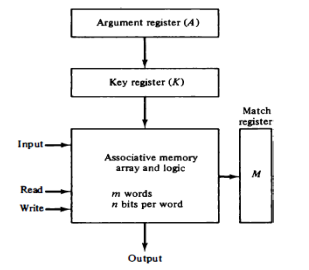
\includegraphics[width=0.7\linewidth]{associative}
    \caption{Associative memory circuit}\label{associative_circuit}
\end{figure}

\section{Associative network}
An associative network is a type of artificial neural network that is designed
to store and retrieve information based on the strength of the connections
between neurons. Associative networks are often used for tasks that require the
recall of specific patterns or relationships, such as image recognition,
natural language processing, and recommendation systems.
\subsection{An Interactive Activation Model of Context Effects in Letter Perception}
\subsubsection{Introduction}
The interactive activation model\cite{auto} is a computational model that
attempts to explain how the brain processes and interprets written language. It
suggests that the brain stores and retrieves information about letters and
words based on the strength of the connections between neurons, and that these
connections are influenced by both bottom-up and top-down processes.

The model proposes that the brain has a hierarchical structure, with
lower-level processing units representing features such as lines and curves,
and higher-level processing units representing letters and words. According to
the model, the activation of a processing unit depends on both the activation
of its inputs and the activation of its outputs.
\subsubsection{Proposed system}
The authors propose a hierarchical structure for the model, with lower-level
processing units representing features such as lines and curves, and
higher-level processing units representing letters and words. They suggest that
the activation of a processing unit depends on both the activation of its
inputs and the activation of its outputs. The main two concepts in this system
are

\begin{description}
    \item[Auto associative memory]A single layer NN in which the number of training
    vectors and the number of output vectors are the same. The weights are
    determined by the stored patterns
    \item[Hetero associative memory]A single layer NN in which the number of input
    training vectors and output are different. Weights are determined by the
    pattern stored in the network. It is static in nature and hence there would be
    no linear or delay operations
\end{description}
\subsubsection{Advantages }
One advantage of the model is that it provides a computational framework for
understanding how the brain processes and interprets written language. It
suggests a hierarchical structure for the brain, with lower-level processing
units representing features such as lines and curves, and higher-level
processing units representing letters and words. Another advantage of the model
is that it is based on the concept of auto-associative and heteroassociative
memory, which are thought to play a role in perception and language processing
in the human brain. This allows the model to capture the complex relationships
between letters and words, and to explain a wide range of phenomena in written
language processing.

\subsubsection{Disadvantages}
A disadvantage of the model is that it is a simplified model of the brain, and
it may not capture all of the complexity and nuance of language processing. It
is also based on a set of assumptions and simplifications, and it may not
accurately reflect the underlying mechanisms of the brain. In addition, the
model is based on a set of equations and learning rules that are used to
simulate the activation and deactivation of processing units, and these
equations may not accurately reflect the underlying mechanisms of the brain.

\subsection{Neural networks and physical systems with emergent collective computational abilities.}
\subsubsection{Introduction}
The Hopfield model\cite{hopfield} is a type of RNN that is designed to mimic
the behaviour of neurons in the brain. It is a type of associative memory
system and hence it can store and recall information based on the relationship
between the data stored. It has applications including pattern recognition,
optimization, and error correction.
\subsubsection{Methodology}
This paper discusses the use of computational models and simulations to study
the behaviour of neural networks and other distributed systems. He proposed an
associative memory network type called the Hopfield network. A Hopfield network
consists of a set of interconnected neurons that are arranged in a single
layer. Each neuron is fully connected in the network, and the connections
between neurons are adjusted based on the strength of the relationships between
the inputs and outputs. The behaviour of a Hopfield network is determined by a
set of equations that describe the activation and deactivation of the neurons
over time. These equations are based on the concept of auto-associative memory,
in which the output is used to retrieve the original input.
\subsubsection{Advantages}
One advantage of the Hopfield model is that it is relatively simple and easy to
implement. It consists of a single layer of interconnected neurons and the
connections between neurons are adjusted based on the strength of the
relationships between the inputs and outputs. This simplicity makes the
Hopfield model easy to understand and implement. Another advantage of the
Hopfield model is that it is capable of storing and retrieving patterns or
sequences of data based on the strength of the connections between neurons.
This makes it useful for tasks that require the recall of specific patterns or
sequences of data, such as image recognition, natural language processing, and
recommendation systems. Also, this model is relatively robust and resistant to
noise. These advantages make it useful in applications like image or speech
recognition systems.
\subsubsection{Disadvantages}
One disadvantage of the Hopfield model is that it is relatively simple and may
not be able to capture the complexity and nuance of more advanced neural
networks. Another drawback is that it can retrieve the information only with
the original input. A third disadvantage of the Hopfield model is that it can
be sensitive to initialization and may not always converge to a stable state
when used with a large amount or insufficiently distinct data. This can make it
difficult to use the model for certain types of tasks, such as optimization or
decision-making.
\section{Spiking neural network}
Spiking neural networks are a type of neural network that models the behaviour
of biological neurons by using spikes or pulses to encode and transmit
information. They are a relatively new type of neural network that has the
potential to improve the performance and efficiency of artificial intelligence
systems. The use of spiking neural networks for building associative memory
systems is a relatively new area of research that has only recently started to
gain attention.

\subsection{SWAT: a spiking neural network training algorithm for classification problems.}
\subsubsection{Introduction}
SWAT\cite{swat}(Spiking Weight association Training) is a method for training
spiking neural networks for classification tasks. It uses a combination of
supervised and unsupervised learning to improve the performance of SNN. It is
based on the idea of adjusting the weights of the connections between neurons
in the network based on the input and output patterns of the network. The
weights are adjusted using a learning rule that takes into account the error
between the actual output of the network and the desired output.
\subsubsection{Methodology}
They propose a method which merges Bienenstock-Cooper-Munro learning
rule(BCM)\cite{bcm} with Spike Time Dependent plasticity Spike-timing-dependent
plasticity (STDP)\cite{stdp}.It yields a unimodal weight distribution where
height is associated with STDP.

The BCM learning rule is based on the idea that the strength of the connections
between neurons in the network should be adjusted based on the activity of the
neurons and the error between the actual output of the network and the desired
output. The rule specifies that the weights of the connections between neurons
should be increased if the activity of the neurons is high and the error is
also high, and the weights should be decreased if the activity of the neurons
is low and the error is also low.

STDP is an unsupervised learning rule based on the functioning of neurons in
the brain for neuromorphic computing, which is the study inspired by the
structure and functioning of the brain. In the process strength of the the
connection between neurons changes based on the relative timing of spikes or
impulses The basic idea behind STDP is that if two $N_{pre}$ and $N_{suc}$
neurons are connected, and their spike time are $t_1$ and $t_2$ respectively
according to STDP \vspace*{-.3pc}
\begin{itemize}
    \item[]Weight of connection from $N_{pre}$ to $N_{suc}$ should  increase, if {\boldmath$t_1>t_2$}
    \item[]Weight of connection from $N_{pre}$ to $N_{suc}$ should  decrease, if {\boldmath$t_1<t_2$}
    \item[]Weight of connection from $N_{pre}$ to $N_{suc}$ should  remain same, if {\boldmath$t_1=t_2$}

\end{itemize}
%\vspace*{-2pc}

Overall SWAT is based on the idea of adjusting the weights of the connections
between neurons in the network based on the input and output patterns of the
network. The weights are adjusted using a learning rule that takes into account
the error between the actual output of the network and the desired output.
\subsubsection{Advantages}
One of the main advantages of SWAT is that it can be used to train spiking
neural networks for classification tasks. This is important because spiking
neural networks are a promising type of artificial neural network that is
thought to have the potential to improve the performance of artificial
intelligence systems. It uses a combination of supervised learning and
unsupervised learning to train the network. This allows the network to learn
from labelled examples as well as identify patterns and features in the data on
its own. Since it is based on the simple learning rules of adjusting the
weights of the connections between neurons in the network based on the input
and output patterns of the network it is relatively easy to implement and
understand. Overall it has the potential to enable the use of SNN in a wide
range of applications
\subsubsection{Disadvantages}
Sometimes this may become computationally intensive, especially for large
networks with many neurons and connections. This could make it difficult to use
SWAT on systems with limited computational resources. Another potential
disadvantage is that it is based on supervised and unsupervised learning, in
which supervised learning requires a large amount of labelled data to train the
network effectively. This may be difficult to obtain in some cases. It also
relies on the initial weights of the connections between neurons in the
network, and these weights may have a significant impact on the performance of
the network. This means that SWAT may be sensitive to initialization and may
require careful tuning of the initial weights to achieve good performance.
\subsection{SpikeProp: backpropagation for networks of spiking neurons.}
\subsubsection{Introduction}
spiking neurons may be more biologically realistic and efficient than other
types of artificial neurons, and they may be more suitable for certain tasks
such as pattern recognition and natural language processing. However, they also
note that training networks of spiking neurons can be difficult due to the
non-differentiable nature of the spiking function. To address this problem, the
authors propose the use of SpikeProp\cite{spikeprop}, which is a method for
training networks of spiking neurons using backpropagation.
\subsubsection{Methodology}
It is a method for training networks of spiking neurons using backpropagation.
The spiking function, which describes the relationship between the input and
the output of a spiking neuron, is not differentiable. This means that
traditional methods for training artificial neural networks, such as
backpropagation, cannot be directly applied to networks of spiking neurons.This
can be avoided by surrogate gradient function that approximates the gradient of
the spiking function, which allows the use of backpropagation to train networks
of spiking neurons.

\subsubsection{Advantages}
It allows the use of backpropagation to train networks of spiking neurons. This
makes it possible to leverage the simplicity and efficiency of backpropagation
for training spiking neural networks. With spikeprop, it is possible to create
artificial neural networks that are more biologically realistic and may be more
suitable for certain tasks. It is also more efficient in training SNN than
other techniques. It makes it effective in applications like image recognition
and language translation.
\subsubsection{Disadvantages}
It is not effective in all applications of spiking neural networks. Due to the
approximations used in surrogate gradient function it may not be always
accurate which may affect its performance
%%********************Chapter 3**********
%==================================introduction.tex=============================
\chapter{Results and Discussion}%

\lipsum[5-7] % Please comment this line and type in the results chapter

\begin{table}[h!]
	\centering
	\caption{test table}
	\vspace*{5pt}
	\begin{tabular}{|c|c|c|}
		\hline
		Sl. No & Item 1 & Itm 2 \\ \hline
		1      & 37     & 45    \\ \hline
		2      & 42     & 23    \\ \hline
		3      & 47     & 1     \\ \hline
		4      & 52     & -21   \\ \hline
		5      & 57     & -43   \\ \hline
		6      & 62     & -65   \\ \hline
		7      & 67     & -87   \\ \hline
		8      & 72     & -109  \\ \hline
		9      & 77     & -131  \\ \hline
		10     & 82     & -153  \\ \hline
	\end{tabular}
\end{table}
%%********************Chapter 4**********
%==================================introduction.tex=============================
\chapter{Conclusion}%

This study presented a method for constructing an associative memory system
using an SNN. This approach combines the principles of associative memory and
SNNs to create a neural network architecture that can store and retrieve
associations between different stimuli.

There are active research going on to develop neuromorphic hardware which
improves the efficiency of different operation involved in the processing of
information using an SNN. The hardware Lohi and software for that Lava are
developed by intel for this application. Software like \textbf NEST and
SpikeTorch is open source tool for the SNN. As more and more research is done
in this field, it could be the next-generation machine learning algorithm.

%%********************References**********
%%****This template uses IEEE bibliography style
%==================================bibiliography.tex================================
\begin{thebibliography}{99}
	\bibitem{india} HU, Yun Chao, et al., \emph{Mobile edge computing?A key technology
		towards 5G}, ETSI white paper, 2015, vol. 11, no 11, p. 1-16.
	
	\bibitem{rpi}
	@online{ Raspberry pi,
		\url{https://www.raspberrypi.org/}
		Online; accessed 10-June-2019
	}

	\bibitem{japan} HU, Yun Chao, et al., \emph{Mobile edge computing?A key technology
		towards 5G}, ETSI white paper, 2015, vol. 11, no 11, p. 1-16.		
	\bibitem{base}He, Hu, et al. "Constructing an Associative Memory System Using Spiking Neural Network." Frontiers in Neuroscience, vol. 13, 2019, https://doi.org/10.3389/fnins.2019.00650.
\end{thebibliography}
"Associative Memory Systems: An Overview" by Y. H. Lee et al., which provides a comprehensive overview of the principles and applications of associative memory systems.

"Spiking Neural Networks: A Comprehensive Introduction" by G. Indiveri et al., which presents a detailed introduction to spiking neural networks, including their properties, applications, and challenges.

"A Spiking Neural Network Model for Robust Associative Memory" by P. V. Klopotek et al., which presents a spiking neural network model for building associative memory systems and discusses its performance and robustness.

"Associative Memory with Spiking Neurons: A Review" by T. Masquelier et al., which provides a review of the existing research on using spiking neurons for building associative memory systems, including a discussion of the benefits and challenges of this approach.
 

\end{document}